\documentclass[12pt,a4paper]{report}

% Packages
\usepackage[utf8]{inputenc}
\usepackage[T1]{fontenc}
\usepackage{amsmath}
\usepackage{amssymb}
\usepackage[lining]{ebgaramond}
\usepackage[cmintegrals,cmbraces]{newtxmath}
\usepackage{microtype}
\usepackage{geometry}
\usepackage{graphicx}
\usepackage{booktabs}
\usepackage{array}
\usepackage{xcolor}
\usepackage{hyperref}
\usepackage{float}
\usepackage{caption}
\usepackage{etoolbox}
\usepackage{enumitem}
\usepackage{makecell}
\graphicspath{{./fig/}}

% Page layout
\geometry{
    left=1.8cm,
    right=1.8cm,
    top=2.2cm,
    bottom=2.2cm
}

% Color definitions
\definecolor{crimson}{RGB}{153, 0, 0}

% Hyperlink settings
\hypersetup{
    colorlinks=true,
    linkcolor=crimson,
    urlcolor=crimson,
    citecolor=crimson
}

\tolerance=2000
\emergencystretch=2em

% Chapter/section title formatting
\usepackage{titlesec}
\titleformat{\chapter}{\normalfont\huge\bfseries}{}{0pt}{}[\vspace{0.3em}]
\titlespacing*{\chapter}{0pt}{0pt}{14pt}
\titleformat{\section}{\normalfont\Large\bfseries}{\thesection}{1em}{}
\titleformat{\subsection}{\normalfont\large\bfseries}{\thesubsection}{1em}{}

\setlength{\parindent}{0pt}
\setlength{\parskip}{4pt}

% Float spacing
\setlength{\floatsep}{6pt plus 2pt minus 2pt}
\setlength{\textfloatsep}{10pt plus 2pt minus 2pt}
\setlength{\intextsep}{10pt plus 2pt minus 2pt}
\setlength{\abovecaptionskip}{4pt}
\setlength{\belowcaptionskip}{0pt}
\captionsetup[figure]{skip=5pt, belowskip=2pt}
\captionsetup[table]{skip=2pt}
\BeforeBeginEnvironment{figure}{\vspace{4pt}}
\AfterEndEnvironment{figure}{\vspace{2pt}}
\AfterEndEnvironment{table}{\vspace{-6pt}}

% Question box: \question{text}
\newcommand{\question}[1]{%
    \hrule
    \vspace{0.2cm}
    #1
    \vspace{0.2cm}
    \hrule
    \vspace{0.5cm}
}

\begin{document}

\pagestyle{plain}

% ─────────────────────────────────────────────
%  Cover Page
% ─────────────────────────────────────────────
\begin{titlepage}
\centering
\vspace*{3cm}

{\fontsize{28}{34}\selectfont\bfseries Digital Communication IC Design\par}
\vspace{0.6em}
{\fontsize{20}{26}\selectfont\bfseries Homework 3\par}

\vspace{1.5cm}
\textcolor{crimson}{\rule{0.6\linewidth}{1.2pt}}
\vspace{1.5cm}

{\large\bfseries Student ID}\par
\vspace{0.4em}
{\large M11407439}\par

\vspace{0.8em}

{\large\bfseries Name}\par
\vspace{0.4em}
{\large MING-HONG, LIN}\par

\vspace{2cm}

{\large\bfseries Development Environment}\par
\vspace{0.8em}
\begin{tabular}{rl}
    \textbf{Language} & MATLAB R2025b \\[4pt]
    \textbf{AI Tool}  & Claude Opus 5.5 \\
\end{tabular}

\vfill

\textcolor{crimson}{\rule{0.6\linewidth}{0.6pt}}\par
\vspace{0.5em}
{\small Due Date: 2026/11/04}

\end{titlepage}

% ─────────────────────────────────────────────
%  Table of Contents
% ─────────────────────────────────────────────
\tableofcontents
\newpage


% ─────────────────────────────────────────────
\chapter{Setup and Code Organization}
% ─────────────────────────────────────────────
My student ID is M11407439, so $m = 39$. This number is only used as the random seed in Q2 and Q4
(\texttt{rng(39, \textquotesingle twister\textquotesingle)}). Everything else in Q1 and Q3 follows from the power delay profile and $F_s = 250$\,MHz.

\begin{table}[H]
\centering
\caption{Files in \texttt{01\_src}}
\setlength{\tabcolsep}{8pt}
\renewcommand{\arraystretch}{1.2}
\begin{tabular}{l>{\raggedright\arraybackslash}p{0.42\linewidth}}
\toprule
\textbf{File} & \textbf{Content} \\
\midrule
\texttt{hw3\_channel.m} & PDP, $p_i$, $\tilde p_i$, $n_i$, and the seed-39 gains $\gamma_i$, $g_i$, $h_i$, $h[n]$ \\
\texttt{ofdm\_size.m}   & Chooses $N_g$ and $N$ from the channel length (Q3) \\
\texttt{q1.m} -- \texttt{q4.m} & One script per question; prints the numbers and saves the figures \\
\makecell[l]{\texttt{new\_fig.m}, \texttt{save\_fig.m}, \\ \texttt{tl\_labels.m}, \texttt{hw\_palette.m}} & Figure style only \\
\bottomrule
\end{tabular}
\end{table}

All four scripts call \texttt{hw3\_channel.m}, so Q2, Q3 and Q4 use exactly the same channel realization. The
numbers in this report are copied from the console output of the scripts.

\newpage

% ─────────────────────────────────────────────
\chapter{Q1 — Power Delay Profile Statistics}
% ─────────────────────────────────────────────
\question{Consider the four-path channel power delay profile below. Use linear power, not dB values, when calculating
channel statistics.
\begin{center}
\begin{tabular}{ccc}
\toprule
Tap $i$ & Power $P_{i,\mathrm{dB}}$ & Delay $\tau_i$ \\
\midrule
0 & 0 dB & 0 ns \\
1 & $-2$ dB & 16 ns \\
2 & $-6$ dB & 92 ns \\
3 & $-9$ dB & 200 ns \\
\bottomrule
\end{tabular}
\end{center}}

\section{(a) Linear and Normalized Powers}

\question{Convert every path power to linear scale, normalize the four powers so that they sum to one, and print both
vectors, $\mathbf{p} = [p_1\ p_2\ p_3\ p_4]$ and $\tilde{\mathbf{p}} = [\tilde p_1\ \tilde p_2\ \tilde p_3\ \tilde p_4]$
with at least six significant digits. (10\%)
\[ p_i = 10^{P_{i,\mathrm{dB}}/10}, \qquad \tilde p_i = \frac{p_i}{\sum_r p_r} \]}

The table numbers the paths from 0 to 3 while the vectors in the question are written from 1 to 4. They describe the
same four paths, so I keep the tap index $i = 0, \ldots, 3$ everywhere; vector entry $j$ is tap $j - 1$.
\texttt{q1.m} prints
\begin{align*}
    \mathbf{p} &= [\,1.00000000 \quad 0.63095734 \quad 0.25118864 \quad 0.12589254\,], && \textstyle\sum_r p_r = 2.0080385, \\
    \tilde{\mathbf{p}} &= [\,0.49799841 \quad 0.31421576 \quad 0.12509155 \quad 0.06269429\,], && \textstyle\sum_r \tilde p_r = 1 .
\end{align*}
The first path is the 0\,dB reference, so $p_0 = 1$ exactly. After normalization it carries almost half of the power,
and the first two paths together hold 81\% of it.

\section{(b) Mean Excess Delay, RMS Delay Spread and Maximum Excess Delay}

\question{Calculate the mean excess delay, RMS delay spread, and maximum excess delay. Show the contribution of each
path to the first and second delay moments. (10\%)
\[ \bar\tau = \sum_i \tilde p_i \tau_i, \qquad \tau_{\mathrm{RMS}} = \sqrt{\sum_i \tilde p_i (\tau_i - \bar\tau)^2} \]}

Table~\ref{tab:q1} lists what each path adds to the first moment $\sum_i \tilde p_i\tau_i$, to the second raw moment
$\sum_i \tilde p_i\tau_i^2$, and to the second central moment $\sum_i \tilde p_i(\tau_i - \bar\tau)^2$.

\begin{table}[H]
\centering
\caption{Power Delay Profile and the Contribution of Each Path to the Delay Moments}
\label{tab:q1}
\setlength{\tabcolsep}{6pt}
\renewcommand{\arraystretch}{1.2}
\begin{tabular}{crcccrrr}
\toprule
$i$ & $P_{i,\mathrm{dB}}$ & $p_i$ & $\tilde p_i$ & $\tau_i$ (ns) & $\tilde p_i \tau_i$ (ns) & $\tilde p_i \tau_i^2$ (ns$^2$) & $\tilde p_i (\tau_i - \bar\tau)^2$ (ns$^2$) \\
\midrule
0 & $0$ dB & 1.00000 & 0.497998 & 0 & 0.0000 & 0.00 & 420.98 \\
1 & $-2$ dB & 0.630957 & 0.314216 & 16 & 5.0275 & 80.44 & 53.71 \\
2 & $-6$ dB & 0.251189 & 0.125092 & 92 & 11.5084 & 1058.77 & 495.31 \\
3 & $-9$ dB & 0.125893 & 0.0626943 & 200 & 12.5389 & 2507.77 & 1831.64 \\
\midrule
Sum & & 2.00804 & 1.00000 & & 29.0747 & 3646.99 & 2801.65 \\
\bottomrule
\end{tabular}

\end{table}

From the sums in the last row,
\begin{align}
    \bar\tau &= \sum_i \tilde p_i \tau_i = 29.0747\ \text{ns}, \\
    \tau_{\mathrm{RMS}} &= \sqrt{\sum_i \tilde p_i(\tau_i - \bar\tau)^2} = \sqrt{2801.65\ \text{ns}^2} = 52.9306\ \text{ns}, \\
    \tau_{\max} &= \tau_3 - \tau_0 = 200\ \text{ns}.
\end{align}
The raw moments give the same spread, $\sqrt{\overline{\tau^2} - \bar\tau^2} = \sqrt{3646.99 - 29.0747^2} =
52.9306$\,ns. For the maximum excess delay I take the last path relative to the first arriving one. All four paths are
within 9\,dB of the strongest, so the common $-10$\,dB threshold would not drop any of them and the answer stays 200\,ns.

The bar charts show how differently the two statistics are built. The first path sits at $\tau = 0$ and adds nothing
to $\bar\tau$, while the weak 200\,ns path ($\tilde p_3 = 0.063$) adds the most, 12.54\,ns. The effect is stronger in
the second central moment, because the distance to $\bar\tau$ is squared: path 3 alone gives 1832 of the 2802\,ns$^2$,
or 65\%, although it holds only 6\% of the power. So $\tau_{\mathrm{RMS}}$ is set mostly by the weak late echo, and it
ends up larger than $\bar\tau$.

\begin{figure}[H]
    \centering
    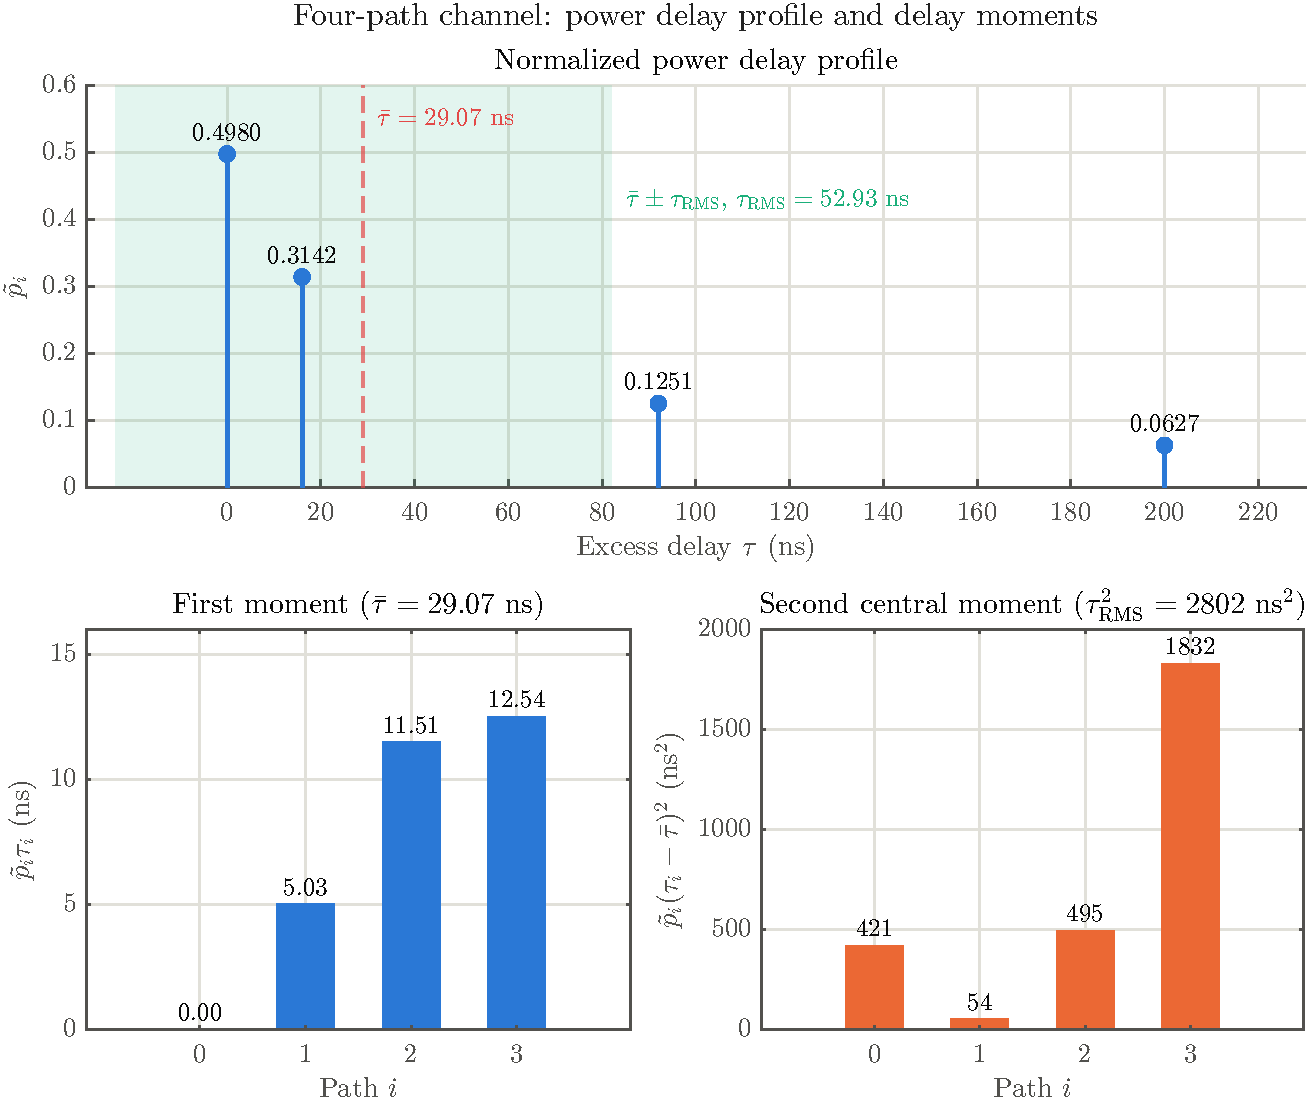
\includegraphics[width=0.92\linewidth]{q1b.pdf}
    \caption{Normalized PDP with $\bar\tau$ (red) and $\bar\tau \pm \tau_{\mathrm{RMS}}$ (green), and the Contribution of Each Path to the First and Second Central Moments}
\end{figure}

\newpage

\section{(c) Coherence Bandwidth}

\question{Using the definition below, calculate the coherence bandwidth. Compare it with signal bandwidths of 2.5 MHz and
250 MHz and classify each channel as approximately flat fading or frequency selective. Explain the criterion. (5\%)
\[ B_c = \frac{1}{5\tau_{\mathrm{RMS}}} \]}

\begin{equation}
    B_c = \frac{1}{5 \times 52.9306\ \text{ns}} = 3.7785\ \text{MHz}.
\end{equation}

\begin{table}[H]
\centering
\caption{Signal Bandwidth Compared with $B_c = 3.78$ MHz}
\setlength{\tabcolsep}{12pt}
\renewcommand{\arraystretch}{1.2}
\begin{tabular}{cccc}
\toprule
$B_s$ & $B_s/B_c$ & Symbol time $1/B_s$ & Classification \\
\midrule
2.5 MHz & 0.66 & 400 ns $\approx 7.6\,\tau_{\mathrm{RMS}}$ & approximately flat fading \\
250 MHz & 66.2 & 4 ns $\approx 0.076\,\tau_{\mathrm{RMS}}$ & frequency selective \\
\bottomrule
\end{tabular}
\end{table}

\textbf{Criterion.} $B_c$ is the frequency separation over which the channel response stays strongly correlated
(course slides Ch.~4, p.~25). If the signal bandwidth is below $B_c$, every frequency component of the signal sees about
the same complex gain, and the channel only scales and rotates the signal. This is flat fading. If $B_s > B_c$,
different parts of the band see different gains and some of them can sit in a deep null, which is frequency-selective
fading. In the time domain the same comparison reads: flat fading when the symbol time is much longer than the delay
spread, and inter-symbol interference when the delay spread is a large part of a symbol or longer.

\textbf{2.5 MHz.} $B_s < B_c$, so I classify it as flat fading. It is only approximately flat, though. The ratio is
0.66, not $\ll 1$, and $K = 5$ is the loose end of the range $K = 5 \sim 50$ given in the slides. With $K = 50$,
$B_c = 378$\,kHz and the same 2.5\,MHz signal would already count as frequency selective. This case is close to the
boundary, and the gain would still tilt a little across the band.

\textbf{250 MHz.} $B_s$ is 66 times $B_c$, so the channel is clearly frequency selective. The band contains many fades
(see $|H(f)|$ in Q2(b), where nulls are a few MHz apart), and a 4\,ns single-carrier symbol would be smeared over about
50 symbols by the 200\,ns channel. This is the case that calls for the OFDM design in Q3 and Q4.

\section{(d) Integer Sample Delays at $F_s = 250$ MHz}

\question{At sampling rate $F_s$ = 250 MHz, convert every path delay to an integer sample delay. Determine the discrete
channel length and the minimum cyclic-prefix length that prevents inter-symbol interference for this channel. (5\%)}

The sample period is $T_s = 1/F_s = 4$\,ns, and every delay is a multiple of it:
\begin{equation}
    n_i = \tau_i F_s = [\,0,\ 16,\ 92,\ 200\,]\ \text{ns} \times 250\ \text{MHz} = [\,0,\ 4,\ 23,\ 50\,].
\end{equation}
No rounding is needed; the largest gap between $\tau_i F_s$ and the integer is $7 \times 10^{-15}$, which is just
floating-point error.

The discrete channel $h[n]$ has nonzero taps at $n = 0, 4, 23, 50$, so its length is
\begin{equation}
    L = \max_i n_i + 1 = 51\ \text{taps}.
\end{equation}
Convolution with $h[n]$ spreads each transmitted sample over the following $L - 1 = 50$ samples. The cyclic prefix has
to absorb this spread, so the minimum CP length is
\begin{equation}
    N_{\mathrm{CP,min}} = L - 1 = 50\ \text{samples} = 200\ \text{ns} = \tau_{\max}.
\end{equation}
Q4(c) confirms that 50 is the exact limit: with a 49-sample CP the channel estimate is already wrong.

\begin{figure}[H]
    \centering
    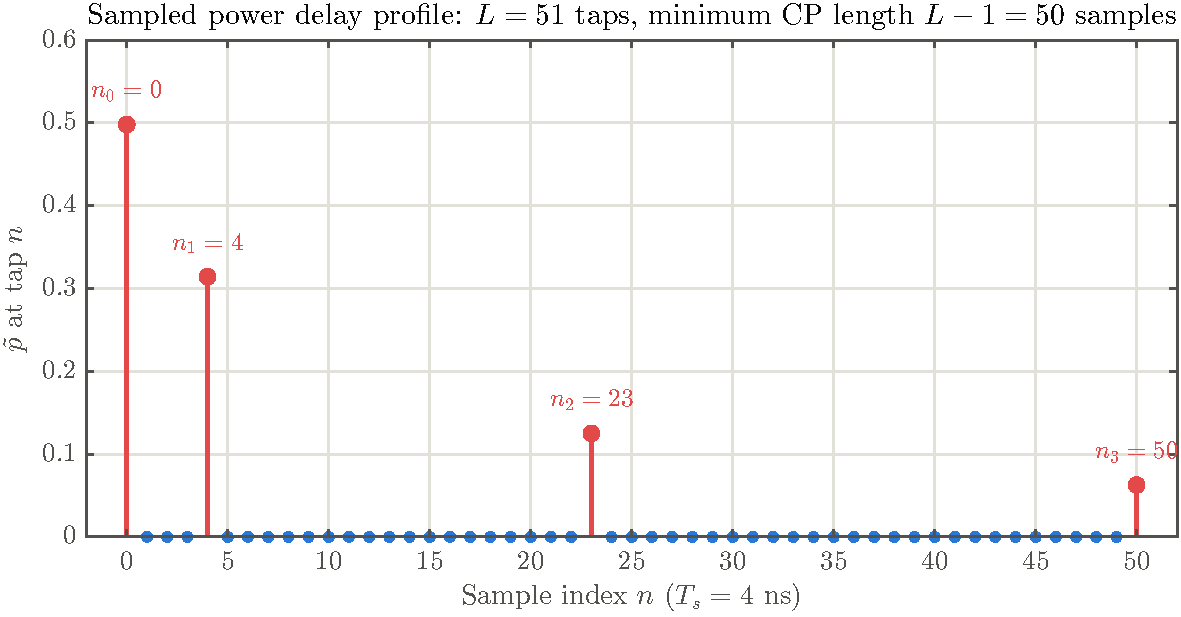
\includegraphics[width=0.9\linewidth]{q1d.pdf}
    \caption{Power Delay Profile on the $F_s = 250$ MHz Sample Grid}
\end{figure}

\newpage

% ─────────────────────────────────────────────
\chapter{Q2 — Random Channel and Its Frequency Response}
% ─────────────────────────────────────────────
\question{Let $m$ be the last two digits of the student ID and use $m$ as the random seed. Generate independent
$\gamma_i$ distributed as $\mathcal{CN}(0,1)$ (complex normal distribution), with real and imaginary components each
having variance 1/2. Use the powers and delays from Question 1.}

\section{(a) Complex Path Gains}

\question{Generate the four complex path gains and normalize them using the equation below. Print $\gamma_i$, $g_i$,
$h_i$, their magnitudes and phases, and the final sum of squared magnitudes. (15\%)
\[ g_i = \sqrt{p_i}\,\gamma_i, \qquad h_i = \frac{g_i}{\sqrt{\sum_r |g_r|^2}} \]}

With \texttt{rng(39, \textquotesingle twister\textquotesingle)} I draw \texttt{gamma = (randn(1,4) + 1j*randn(1,4))/sqrt(2)}, so the real and
imaginary parts are independent $\mathcal{N}(0, 1/2)$ and $E|\gamma_i|^2 = 1$. Table~\ref{tab:q2a} lists the results
(the console prints six decimals; four are kept here).

\begin{table}[H]
\centering
\caption{Path Gains $\gamma_i$, $g_i$ and $h_i$ with Their Magnitudes and Phases}
\label{tab:q2a}
\setlength{\tabcolsep}{3pt}
\renewcommand{\arraystretch}{1.25}
\footnotesize
\begin{tabular}{c|rr|rr|rr}
\toprule
$i$ & \multicolumn{2}{c|}{$\gamma_i$} & \multicolumn{2}{c|}{$g_i = \sqrt{p_i}\,\gamma_i$} & \multicolumn{2}{c}{$h_i$} \\
 & value & $|\cdot|$, $\angle\cdot$ (rad) & value & $|\cdot|$, $\angle\cdot$ (rad) & value & $|\cdot|$, $\angle\cdot$ (rad) \\
\midrule
0 & $0.0190 + 0.2488j$ & $0.2495$, $1.4947$ & $0.0190 + 0.2488j$ & $0.2495$, $1.4947$ & $0.0203 + 0.2664j$ & $0.2672$, $1.4947$ \\
1 & $0.9222 + 0.0498j$ & $0.9235$, $0.0540$ & $0.7325 + 0.0396j$ & $0.7336$, $0.0540$ & $0.7846 + 0.0424j$ & $0.7857$, $0.0540$ \\
2 & $0.5923 - 0.0540j$ & $0.5947$, $-0.0909$ & $0.2968 - 0.0271j$ & $0.2981$, $-0.0909$ & $0.3180 - 0.0290j$ & $0.3193$, $-0.0909$ \\
3 & $-1.2012 - 0.0768j$ & $1.2037$, $-3.0777$ & $-0.4262 - 0.0273j$ & $0.4271$, $-3.0777$ & $-0.4565 - 0.0292j$ & $0.4575$, $-3.0777$ \\
\midrule
$\sum|\cdot|^2$ & \multicolumn{2}{c|}{2.717686} & \multicolumn{2}{c|}{0.871620} & \multicolumn{2}{c}{1.000000} \\
\bottomrule
\end{tabular}

\end{table}

The final sum is $\sum_i |h_i|^2 = 1.000000000000000$.

Multiplying by $\sqrt{p_i} > 0$ and dividing by a positive constant only changes magnitudes, so $\gamma_i$, $g_i$ and
$h_i$ share the same phase. The question uses $p_i$ rather than $\tilde p_i$ inside $g_i$. This does not change $h_i$:
$\tilde p_i = p_i/\sum_r p_r$ only adds a common factor, and the normalization removes it again.

The powers of this realization, $|h_i|^2 = [0.071,\ 0.617,\ 0.102,\ 0.209]$, are quite different from the average
profile $\tilde p_i = [0.498,\ 0.314,\ 0.125,\ 0.063]$. Path 0 happened to fall into a fade ($|\gamma_0| = 0.25$) and
path 3 got a large draw ($|\gamma_3| = 1.20$). That is normal for Rayleigh fading: the PDP only fixes $E|h_i|^2$, and
one snapshot can look very different from the average.

\newpage

\section{(b) Continuous Frequency Response}

\question{The continuous-time impulse response is given as follows. Derive its continuous-frequency response. Draw the
frequency domain response including magnitude and phase versus frequency. Note that the frequency range should cover
$-250$\,MHz to 250\,MHz. (15\%)
\[ h(t) = \sum_{i=0}^{3} h_i\,\delta(t - \tau_i) \]}

A delayed impulse transforms into a linear-phase exponential, $\mathcal{F}\{\delta(t - \tau_i)\} =
e^{-j2\pi f\tau_i}$, and the Fourier transform is linear, so
\begin{equation}
    H(f) = \int_{-\infty}^{\infty} h(t)\,e^{-j2\pi f t}\,dt
         = \sum_{i=0}^{3} h_i\,e^{-j2\pi f \tau_i}
         = h_0 + h_1 e^{-j2\pi f (16\,\mathrm{ns})} + h_2 e^{-j2\pi f (92\,\mathrm{ns})} + h_3 e^{-j2\pi f (200\,\mathrm{ns})} .
\end{equation}
Writing each gain in polar form, $h_i = |h_i|e^{j\theta_i}$ with $\theta_i = \angle h_i$ from Table~\ref{tab:q2a}, the
real and imaginary parts are
\begin{equation}
    \mathrm{Re}\,H(f) = \sum_{i=0}^{3} |h_i| \cos(\theta_i - 2\pi f\tau_i), \qquad
    \mathrm{Im}\,H(f) = \sum_{i=0}^{3} |h_i| \sin(\theta_i - 2\pi f\tau_i),
\end{equation}
so the magnitude and phase plotted below are
\begin{equation}
    |H(f)| = \sqrt{\big(\mathrm{Re}\,H(f)\big)^2 + \big(\mathrm{Im}\,H(f)\big)^2}, \qquad
    \angle H(f) = \operatorname{atan2}\big(\mathrm{Im}\,H(f),\ \mathrm{Re}\,H(f)\big) \in (-\pi, \pi].
\end{equation}
I evaluate them on a 50\,kHz grid from $-250$ to 250\,MHz.

$H(f)$ is a sum of four phasors that turn at different rates as $f$ changes. Where they line up, $|H(f)|$ reaches
1.83; where they cancel, it drops to 0.007 ($-43$\,dB, at $-43.95$\,MHz). The fastest phasor belongs to the 200\,ns
path and makes one turn every $1/200\,\text{ns} = 5$\,MHz, which sets the fine ripple in the plot. Near each deep null
the phase jumps by almost $\pi$, because $H(f)$ passes close to the origin. Between nulls the phase falls steadily with
$f$, as the $e^{-j2\pi f\tau_i}$ terms predict.

\begin{figure}[H]
    \centering
    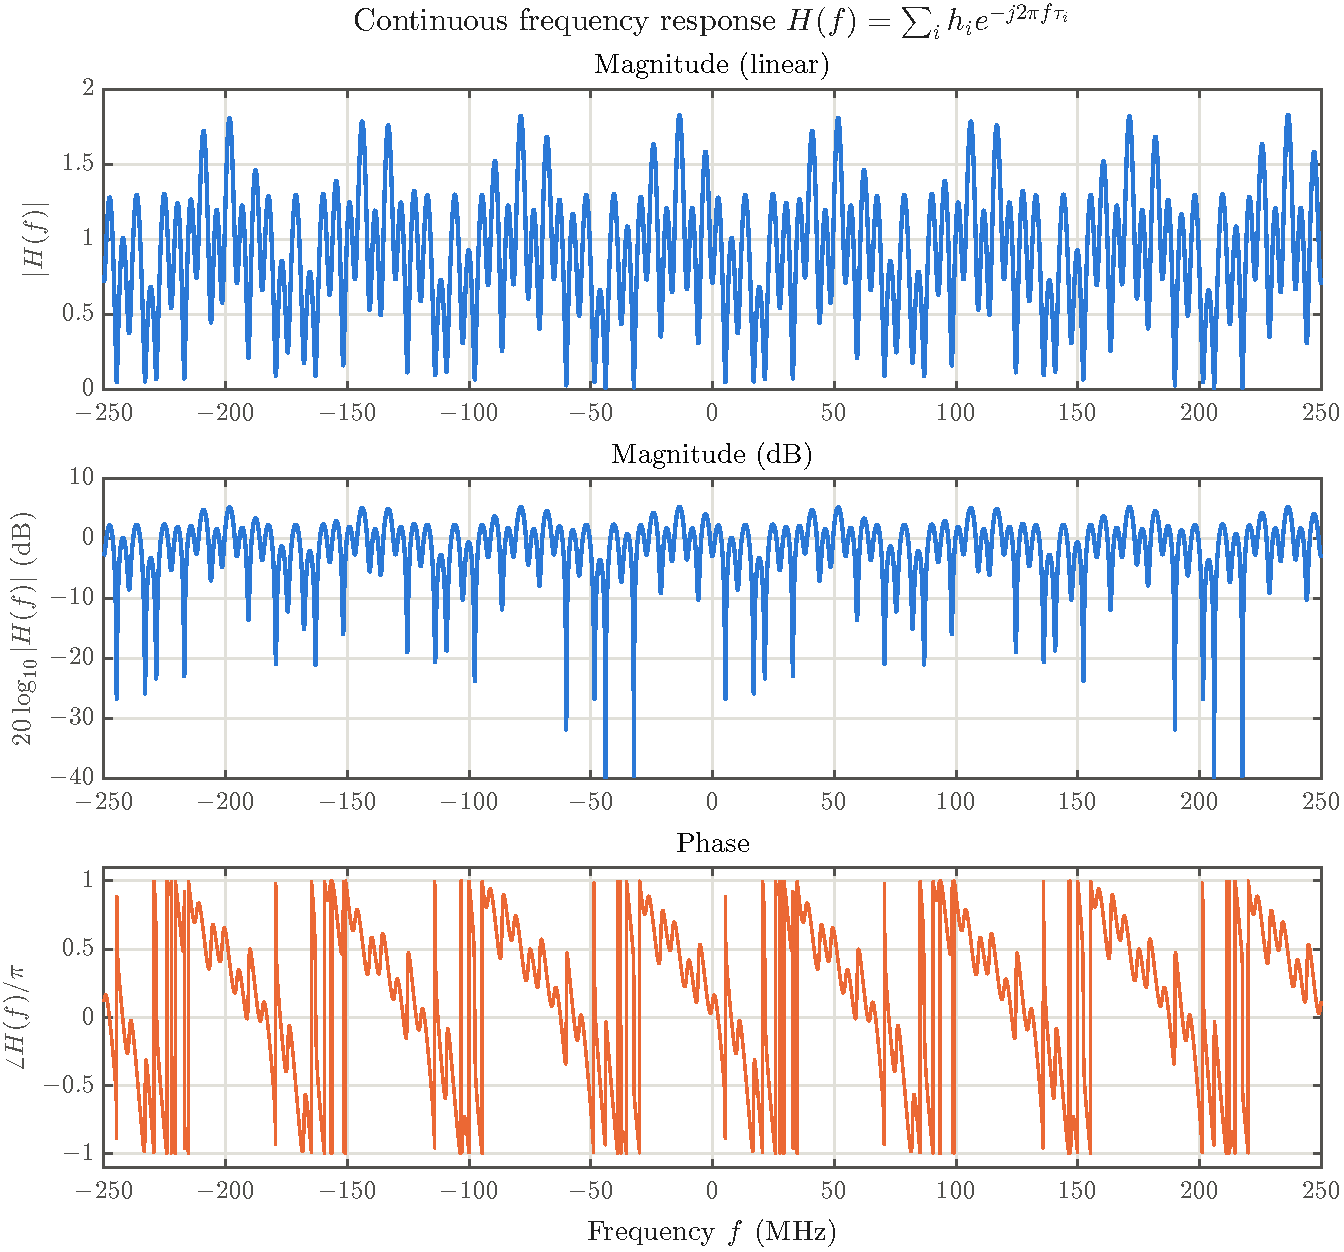
\includegraphics[width=0.92\linewidth]{q2b.pdf}
    \caption{Magnitude (Linear and dB) and Phase of $H(f)$ from $-250$ to 250 MHz}
\end{figure}

\newpage

\section{(c) Verification and Periodicity}

\question{How do you verify your figure in Q2(b)? Do you observe any periodicity? Please state the reasons for the
periodicity or non-periodicity of the figure. (10\%)}

\textbf{Verification.} I checked the figure in three independent ways.
\begin{enumerate}[label=\arabic*)]
    \item \emph{FFT of the sampled channel.} Every $\tau_i$ is a whole number of samples ($\tau_i = n_i T_s$), so
    $H(f) = \sum_i h_i e^{-j2\pi f n_i/F_s}$ is exactly the DTFT of $h[n]$ at $\omega = 2\pi f/F_s$. A 200-point FFT
    of $h[n]$ samples this DTFT every 1.25\,MHz. In the figure below the circles sit on the closed-form curve in both
    magnitude and phase; the largest difference over 401 points is $1.5 \times 10^{-14}$.
    \item \emph{Closed-form values.} At $f = 0$ all exponentials equal 1, so $H(0) = \sum_i h_i = 0.6664 + 0.2506j$,
    which matches the plot ($|H(0)| = 0.712$). Parseval gives a second check. Averaged over one period, the cross
    terms $h_i h_r^* e^{-j2\pi f(\tau_i - \tau_r)}$ vanish and $\overline{|H(f)|^2} = \sum_i |h_i|^2 = 1$. The
    numerical mean is 1.000000, which is also why $|H(f)|$ moves around 1 in the plot.
    \item \emph{Periodicity test,} explained next.
\end{enumerate}

\textbf{Periodicity.} Yes. The curve from $-250$ to 0\,MHz repeats exactly from 0 to 250\,MHz, in magnitude and in
phase, so $H(f)$ is periodic with period 250\,MHz. The bottom panel overlays $|H(f)|$ on $[-250, 0]$ with
$|H(f + 250\ \text{MHz})|$; the two curves coincide, with a largest difference of $2.0 \times 10^{-14}$.

The reason is that all delays are integer multiples of a common delay. $H(f + P) = H(f)$ for every $f$ requires
$e^{-j2\pi P\tau_i} = 1$ for every path, i.e.\ $P\tau_i$ must be an integer for all $i$. The largest delay unit shared
by all paths is
\begin{equation}
    \gcd(16, 92, 200)\ \text{ns} = 4\ \text{ns} = T_s
    \qquad\Rightarrow\qquad
    P = \frac{1}{\gcd(\tau_i)} = \frac{1}{4\ \text{ns}} = 250\ \text{MHz} = F_s .
\end{equation}
250\,MHz is also the \emph{smallest} period. In samples the delays are 4, 23 and 50, and $\gcd(4, 23, 50) = 1$, so no
shorter $P$ makes all three products integers. The script checks this as well: shifting by 125\,MHz or 62.5\,MHz
leaves errors of 0.64 and 1.37. The same holds for $|H(f)|$ alone, since $|H(f)|^2$ contains the differences
$\tau_i - \tau_r$, whose gcd is again 4\,ns.

From the sampling point of view this is the familiar rule that a discrete-time signal has a $2\pi$-periodic spectrum.
All taps lie on the 4\,ns grid, so the channel acts like the discrete filter $h[n]$ and its response repeats every
$F_s$. The required range of $\pm 250$\,MHz therefore shows exactly two periods. If one delay were off the common grid
(say an irrational ratio such as 16\,ns and $10\sqrt 2$\,ns), no common period would exist and $H(f)$ would never repeat
exactly.

What the figure does \emph{not} have is mirror symmetry: $|H(-f)| \neq |H(f)|$, with differences up to 0.62. A real
impulse response would give $H(-f) = H^*(f)$, but the baseband gains $h_i$ are complex, so that symmetry does not apply.

\begin{figure}[H]
    \centering
    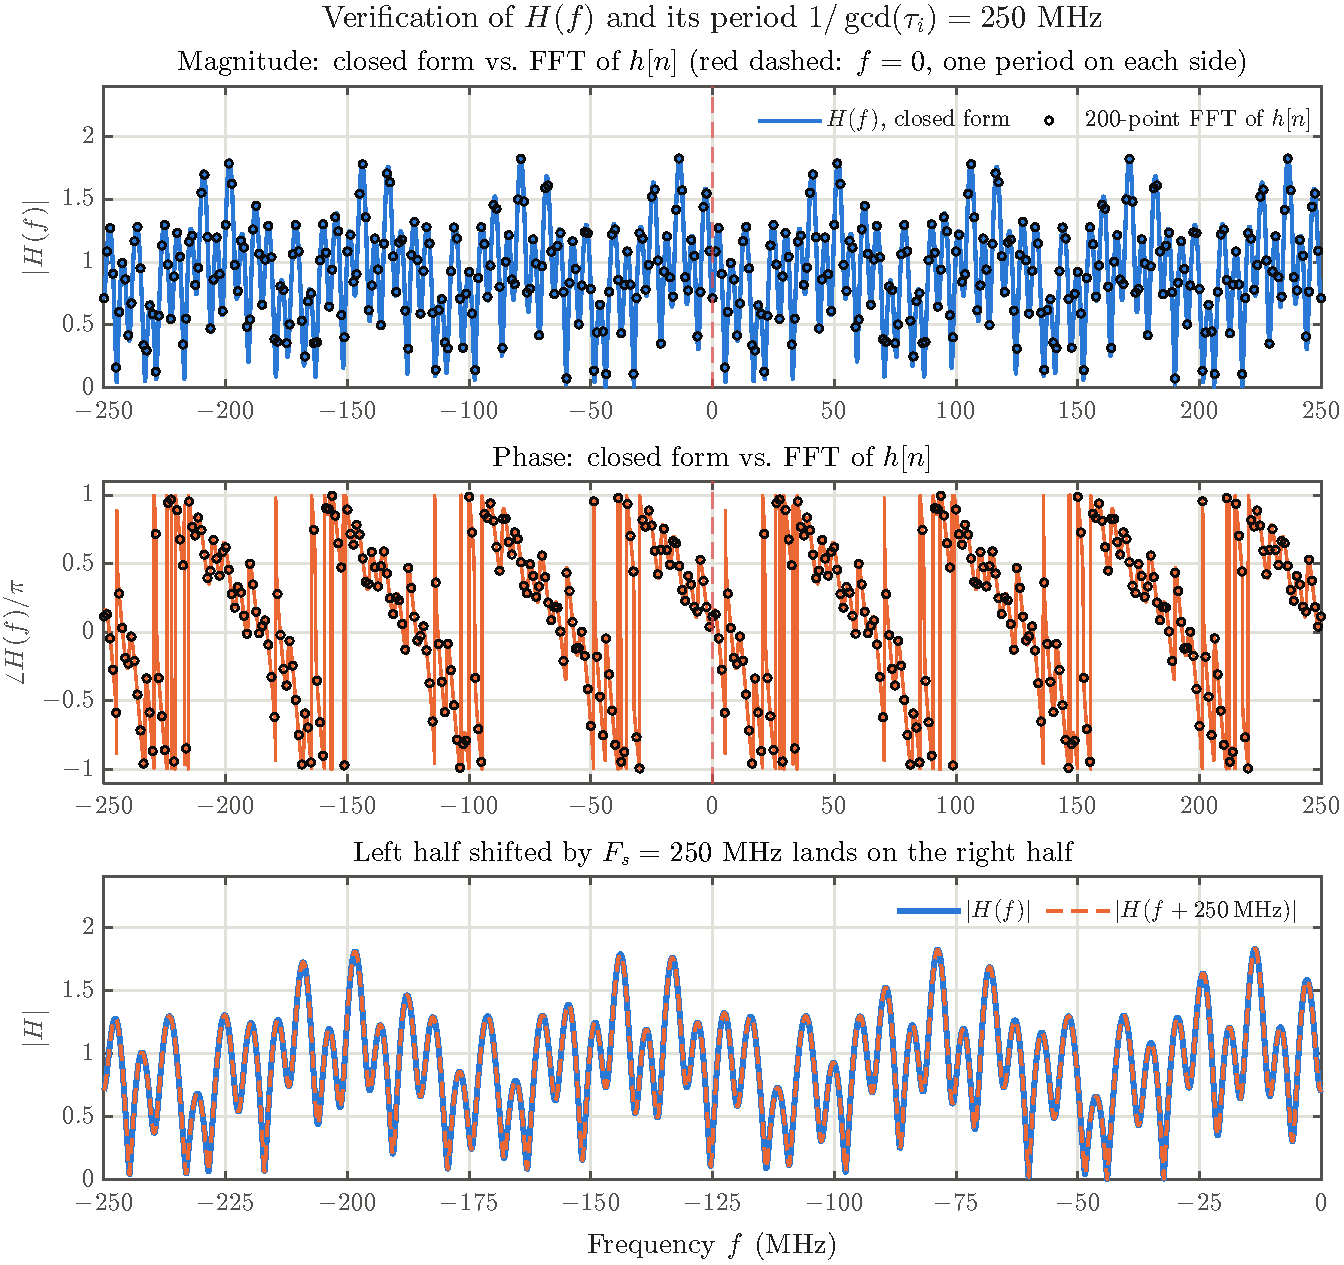
\includegraphics[width=0.92\linewidth]{q2c.pdf}
    \caption{Verification of $H(f)$: Closed Form vs.\ FFT of $h[n]$ (top, middle) and $|H(f)|$ vs.\ $|H(f + 250\ \mathrm{MHz})|$ (bottom)}
\end{figure}

\newpage

% ─────────────────────────────────────────────
\chapter{Q3 — OFDM System Design}
% ─────────────────────────────────────────────
\question{Use $F_s$ = 250 MHz and the time-invariant discrete channel from Question 2 to design an OFDM system.}

\section{(a) Guard Interval}

\question{Determine the minimum guard interval length to prevent ISI, and select an appropriate $N_g$ value that is a
power of 2. (10\%)}

The discrete channel from Q2 is $h[n] = \sum_i h_i\,\delta[n - n_i]$ with $n_i = 0, 4, 23, 50$, so its memory is
$L - 1 = 50$ samples. The guard interval must cover this memory; otherwise the tail of one OFDM symbol runs into the
useful part of the next one:
\begin{equation}
    N_{g,\min} = L - 1 = 50\ \text{samples} = 200\ \text{ns}.
\end{equation}
The powers of 2 next to 50 are 32 and 64. 32 is too short, so I choose
\begin{equation}
    N_g = 64\ \text{samples} = 256\ \text{ns},
\end{equation}
which leaves 14 samples (56\,ns) of margin, for example against timing errors.

\section{(b) FFT Size}

\question{If the guard interval ratio should be smaller than 1/4, what is the proper setting of FFT size $N$ in an OFDM
system. Select the minimum value to satisfy the constraint. (5\%)}

$N_g/N < 1/4$ means $N > 4N_g = 256$, and the FFT size is a power of 2:

\begin{table}[H]
\centering
\caption{Guard Interval Ratio for $N_g = 64$}
\setlength{\tabcolsep}{14pt}
\renewcommand{\arraystretch}{1.2}
\begin{tabular}{ccc}
\toprule
$N$ & $N_g/N$ & $< 1/4$ ? \\
\midrule
128 & 1/2 & no \\
256 & 1/4 & no (equal, not smaller) \\
\textbf{512} & \textbf{1/8} & \textbf{yes} \\
\bottomrule
\end{tabular}
\end{table}

$N = 256$ gives exactly 1/4, which is not smaller than 1/4, so the minimum FFT size is
\begin{equation}
    N = 512, \qquad \frac{N_g}{N} = \frac{1}{8}, \qquad \Delta f = \frac{F_s}{N} = 488.28\ \text{kHz}.
\end{equation}
One OFDM symbol is $N + N_g = 576$ samples: 2048\,ns of useful time plus a 256\,ns CP, so the CP costs
$64/576 = 11.1\%$ of the air time. The subcarrier spacing of 488\,kHz is about 7.7 times smaller than $B_c = 3.78$\,MHz
from Q1(c), so each subcarrier on its own sees an almost flat channel. This is the whole idea of OFDM.

\section{(c) Channel Response at the Subcarriers}

\question{Now calculate the subcarrier frequency $f_k$ in the frequency domain for $k = -N/2 \sim N/2 - 1$. Draw the
frequency domain response at each subcarrier of the channel described in Q2. Note that the frequency response should
include both phase and magnitude. Please use stem plots. (10\%)}

The subcarrier frequencies are
\begin{equation}
    f_k = k\,\Delta f = k\,\frac{F_s}{N}, \qquad k = -256, \ldots, 255,
    \qquad f_k \in [-125,\ 124.51]\ \text{MHz},
\end{equation}
and the channel response at each of them follows from Q2(b):
\begin{equation}
    H[k] = H(f_k) = \sum_{i=0}^{3} h_i\,e^{-j2\pi f_k \tau_i} = \sum_{i=0}^{3} h_i\,e^{-j2\pi k n_i/N}.
\end{equation}
The second form shows that $H[k]$ is also the $N$-point DFT of $h[n]$, with $k$ reordered to $-N/2 \sim N/2-1$. The
script finds the two equal to within $7.9 \times 10^{-15}$. Table~\ref{tab:q3c} lists some of the 512 subcarriers: both
band edges, the strongest and weakest ones, and the ones around DC.

\begin{table}[H]
\centering
\caption{Selected Subcarrier Frequencies and Channel Values ($\Delta f = 488.28125$ kHz)}
\label{tab:q3c}
\setlength{\tabcolsep}{14pt}
\renewcommand{\arraystretch}{1.15}
\begin{tabular}{rrcc}
\toprule
$k$ & $f_k$ (MHz) & $|H[k]|$ & $\angle H[k]$ (rad) \\
\midrule
$-256$ & $-125.000000$ & 0.3101 & $1.4725$ \\
$-255$ & $-124.511719$ & 0.6369 & $1.3833$ \\
$-128$ & $-62.500000$ & 1.2326 & $0.0163$ \\
$-90$ & $-43.945312$ & 0.0090 & $-0.4678$ \\
$-28$ & $-13.671875$ & 1.8275 & $1.4827$ \\
$-1$ & $-0.488281$ & 0.7685 & $0.1584$ \\
$0$ & $0.000000$ & 0.7119 & $0.3598$ \\
$1$ & $0.488281$ & 0.8143 & $0.5035$ \\
$128$ & $62.500000$ & 1.4476 & $0.4703$ \\
$255$ & $124.511719$ & 0.1320 & $-0.0012$ \\
\bottomrule
\end{tabular}

\end{table}

In the figure the stems sample the gray curve, which is the continuous $|H(f)|$ and $\angle H(f)$ of Q2(b) on the same
axis. The subcarriers cover exactly one period $[-F_s/2, F_s/2)$ of $H(f)$, i.e.\ the middle half of the Q2(b) plot.
Since $\Delta f = 488$\,kHz is much finer than the 5\,MHz ripple, the stems follow every peak and null. The strongest
subcarrier is $k = -28$ ($|H| = 1.83$) and the weakest is $k = -90$ ($|H| = 0.009$, almost a null). Neighboring
subcarriers differ only a little, which is the per-subcarrier flatness mentioned in (b).

\begin{figure}[H]
    \centering
    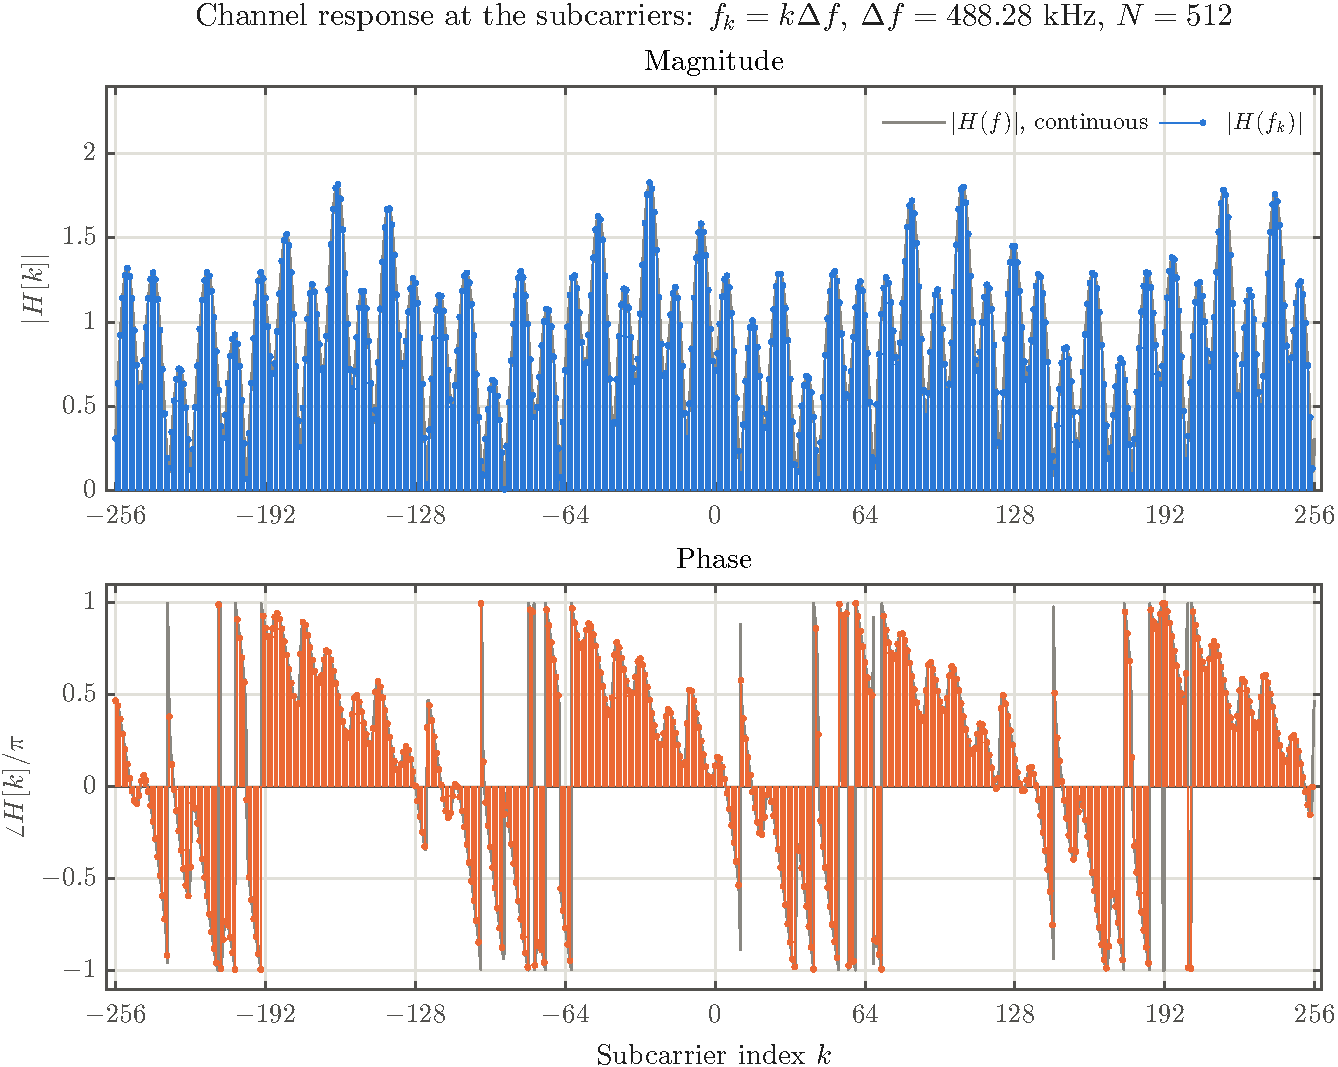
\includegraphics[width=0.92\linewidth]{q3c.pdf}
    \caption{Magnitude and Phase of $H[k] = H(f_k)$ at the $N = 512$ Subcarriers (stems) with the Continuous $H(f)$ (gray)}
\end{figure}

\newpage

% ─────────────────────────────────────────────
\chapter{Q4 — OFDM Transmission over the Channel}
% ─────────────────────────────────────────────
\question{Now, let transmit the OFDM signal through the channel. Use the parameters calculated in Q3.}

Everything in Q4 uses $N = 512$ and $N_g = 64$ from Q3, and the channel $h[n]$ of Q2 ($L = 51$).

\section{(a) QPSK Data, IFFT and Cyclic Prefix}

\question{Please randomly generate frequency domain data from QPSK constellation (black constellation points in
Homework 1). Draw the real part and imaginary part of frequency domain data $X[k]$ versus subcarrier index. Then
transform it to time domain and add the cyclic prefix with length specified in Q3, which is indicated by $x[n]$. (10\%)}

The black points of HW1 Fig.~1 lie at $45^\circ$, $135^\circ$, $225^\circ$ and $315^\circ$ on the unit circle. As in
HW1, the two bits $(b_0, b_1)$ assigned to subcarrier $k$ map to
\begin{equation}
    X[k] = \frac{(1 - 2b_0) + j(2b_1 - 1)}{\sqrt 2},
\end{equation}
i.e.\ $(0,1) \to e^{j\pi/4}$, $(1,1) \to e^{j3\pi/4}$, $(1,0) \to e^{j5\pi/4}$ and $(0,0) \to e^{j7\pi/4}$.
I draw $2N = 1024$ random bits with \texttt{randi}, continuing the seed-39 stream after the four $\gamma_i$, and put
one symbol on each subcarrier $k = -256, \ldots, 255$. The four symbols occur 162, 120, 120 and 110 times. Every $X[k]$
has $|X[k]| = 1$, so its real and imaginary parts only take the values $\pm 1/\sqrt 2$ (Figure~\ref{fig:q4a1}). With
512 stems the full-band panels are dense, so the bottom row of that figure zooms into $k = -16 \sim 15$, where each
symbol can be read off.

For the transform I use the unitary DFT pair
\begin{equation}
    x[n] = \frac{1}{\sqrt N}\sum_{k=-N/2}^{N/2-1} X[k]\,e^{j2\pi kn/N}, \qquad
    Y[k] = \frac{1}{\sqrt N}\sum_{n=0}^{N-1} y[n]\,e^{-j2\pi kn/N},
\end{equation}
implemented as \texttt{sqrt(N)*ifft(ifftshift(X))} and \texttt{fftshift(fft(y))/sqrt(N)}. This keeps the average power
of $x[n]$ at 1, the same as $X[k]$; any matching pair of scalings would give the same $H[k]$ in (c). The CP is the last
$N_g = 64$ samples copied to the front:
\begin{equation}
    x_{\mathrm{cp}}[n] = [\,x[N - N_g], \ldots, x[N-1],\ x[0], \ldots, x[N-1]\,], \qquad 576\ \text{samples}.
\end{equation}
In Figure~\ref{fig:q4a2} the gray block ($n = 0 \sim 63$) is the CP and the green block ($n = 512 \sim 575$) is where it
was copied from; the difference between them is exactly 0. The time signal looks like noise with a peak of
$|x| = 2.59$, as expected for 512 subcarriers with random phases.

\begin{figure}[H]
    \centering
    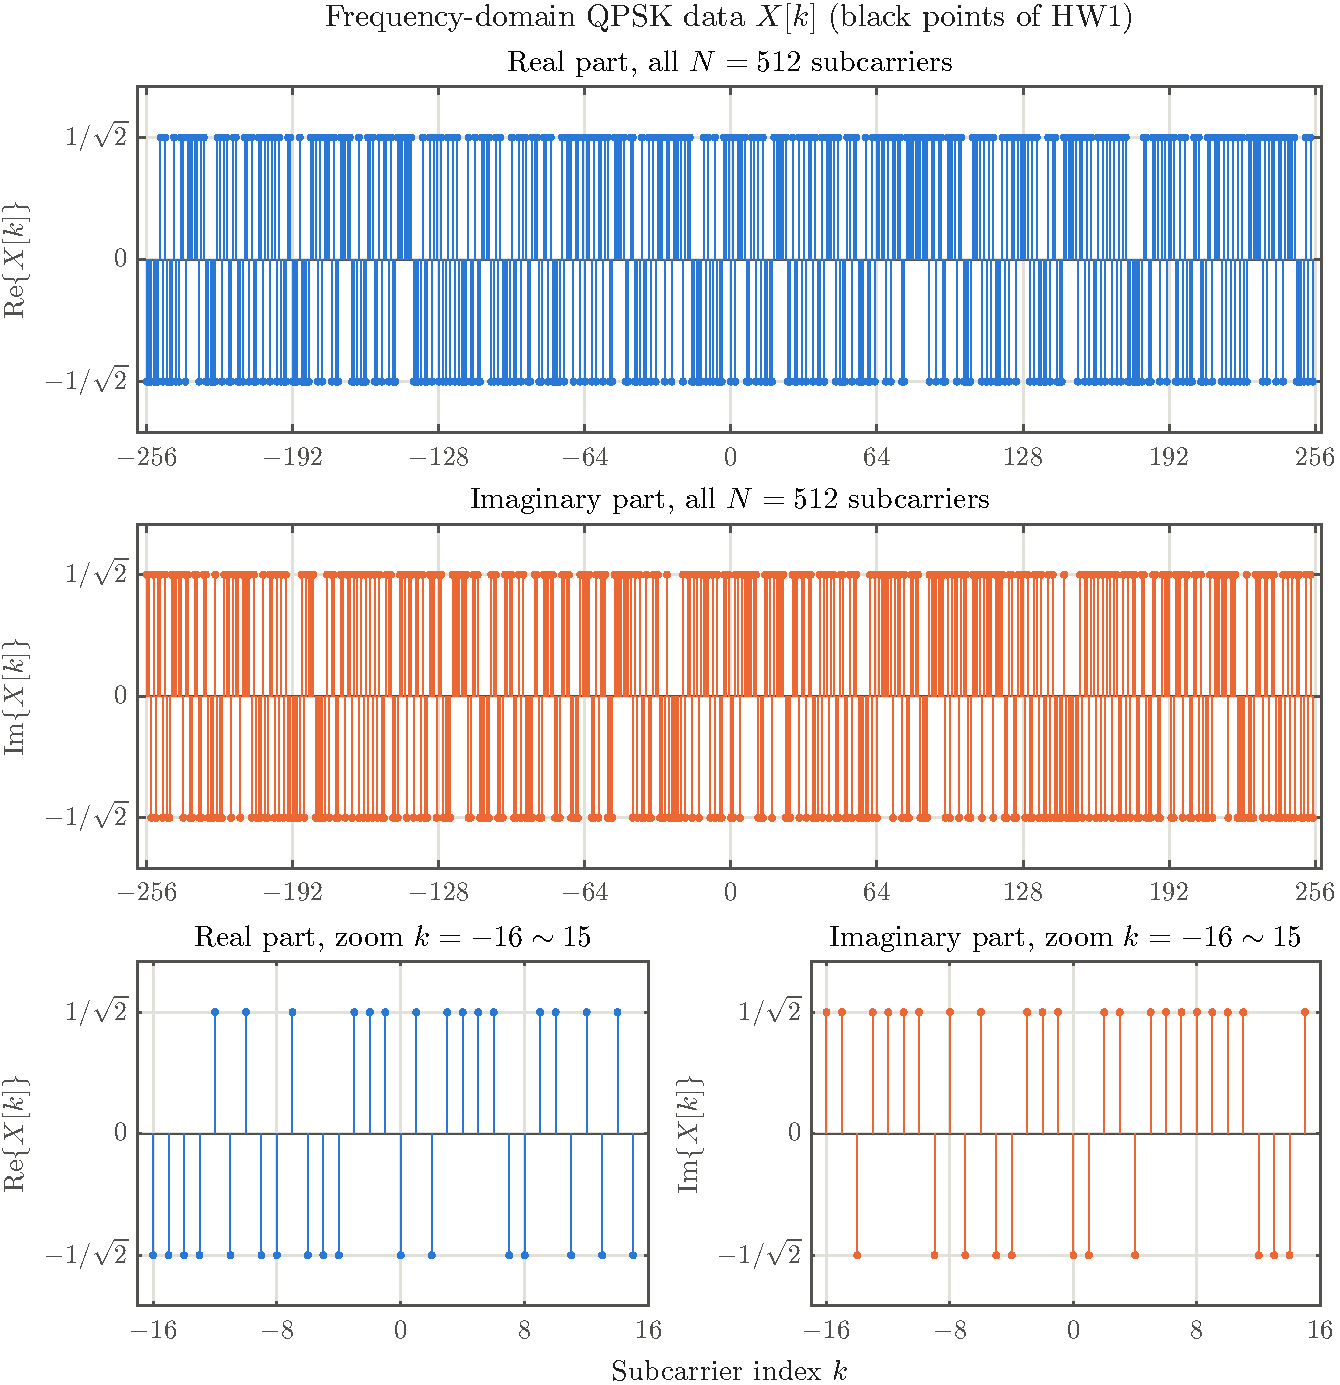
\includegraphics[width=0.88\linewidth]{q4a1.pdf}
    \caption{Real and Imaginary Parts of the QPSK Data $X[k]$ versus Subcarrier Index (bottom: zoom on $k = -16 \sim 15$)}
    \label{fig:q4a1}
\end{figure}

\begin{figure}[H]
    \centering
    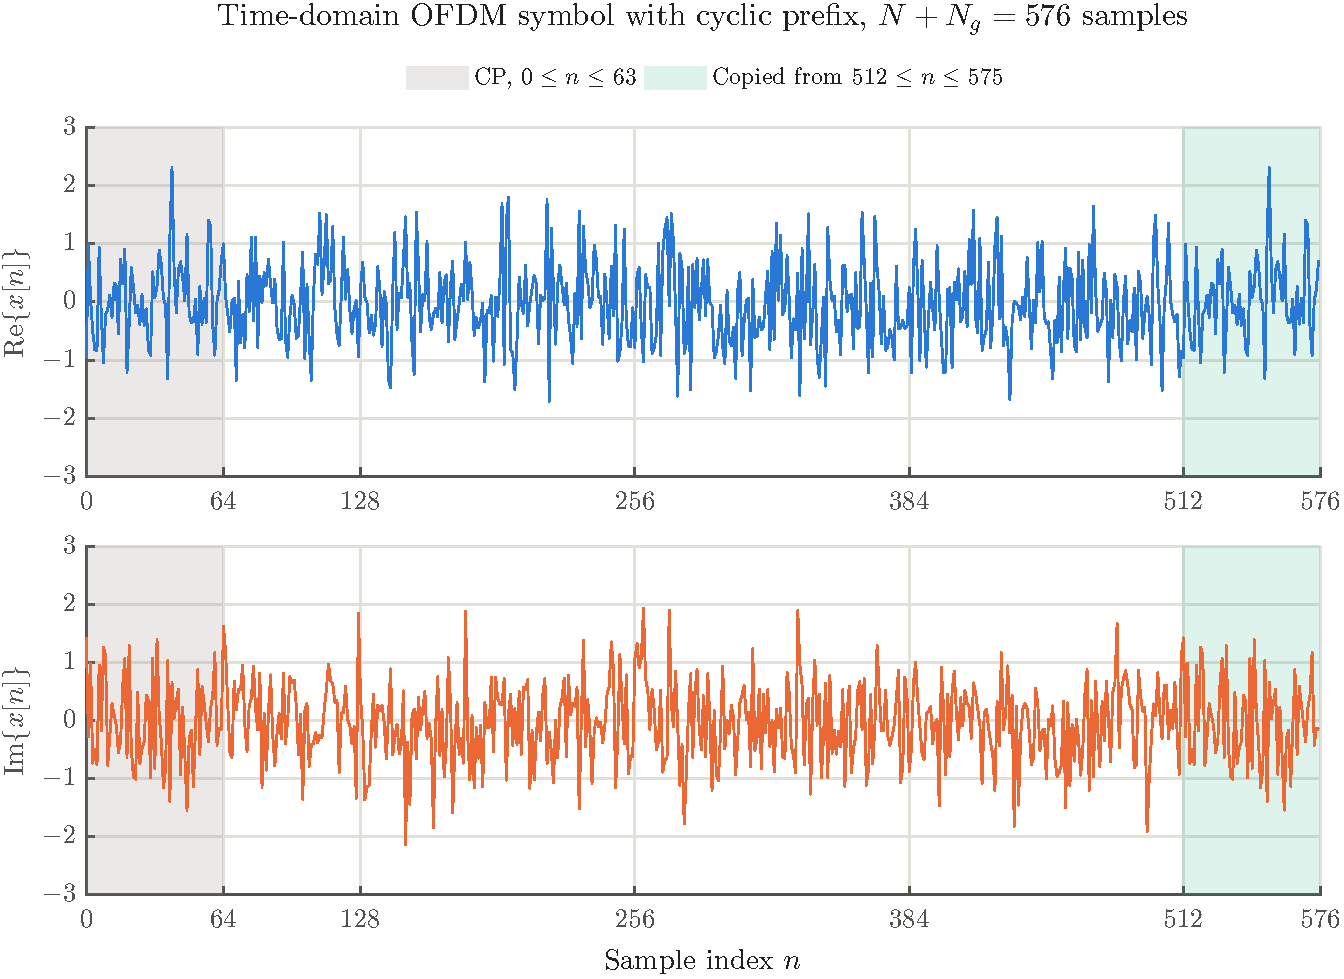
\includegraphics[width=0.92\linewidth]{q4a2.pdf}
    \caption{Real and Imaginary Parts of the Transmitted Signal $x[n]$ with Cyclic Prefix}
    \label{fig:q4a2}
\end{figure}

\newpage

\section{(b) Received Signal}

\question{Use your own channel generated in Q2. Assume the discrete-time channel impulse response is described by
\[ h[n] = \sum_{i=0}^{3} h_i\,\delta[n - n_i], \qquad n_i = \tau_i F_s . \]
Then generate the received signal $y[n] = h[n] \otimes x[n]$, where $\otimes$ denotes linear convolution. Then, draw the
real-part and imaginary-part of your time-domain received signal first. Remove CP, transform it back to frequency domain
by DFT to obtain $Y[k]$. Draw the magnitude of your frequency domain signal versus subcarrier index. (10\%)}

\texttt{conv(hn, xcp)} returns $51 + 576 - 1 = 626$ samples. In the figure below, the first 64 (gray) are the CP region
and get removed. The last 50 (red) are the channel tail, i.e.\ echoes of the end of the symbol that arrive after the
transmitter has stopped. In a continuous stream this tail would land on the CP of the \emph{next} symbol, which is
thrown away as well; this is how the CP blocks ISI. The receiver keeps $n = 64 \sim 575$ and takes the DFT.

\begin{figure}[H]
    \centering
    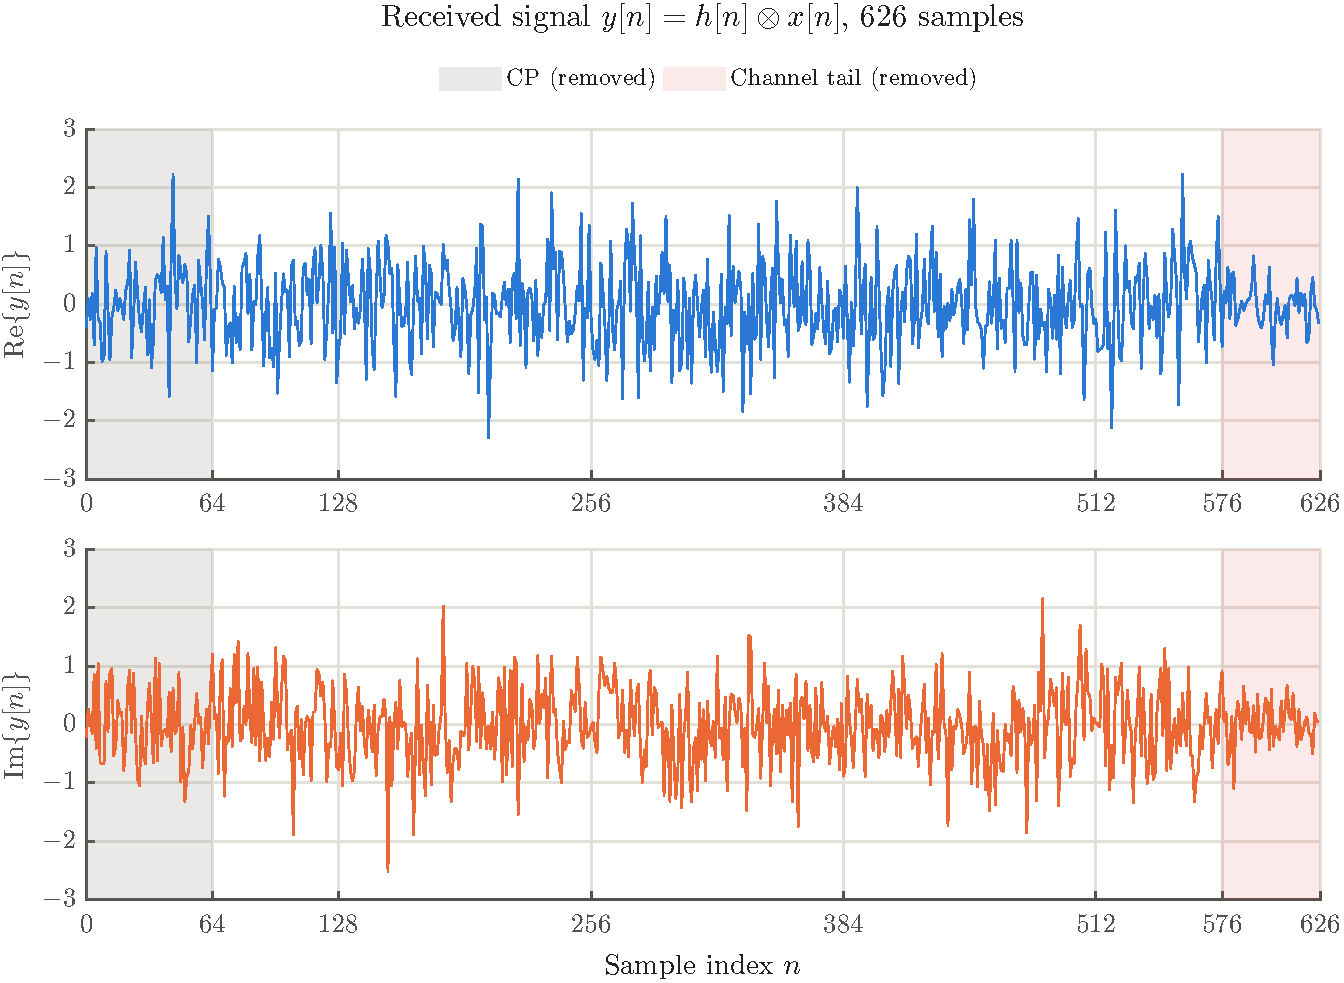
\includegraphics[width=0.92\linewidth]{q4b1.pdf}
    \caption{Real and Imaginary Parts of the Received Signal $y[n]$}
\end{figure}

\begin{figure}[H]
    \centering
    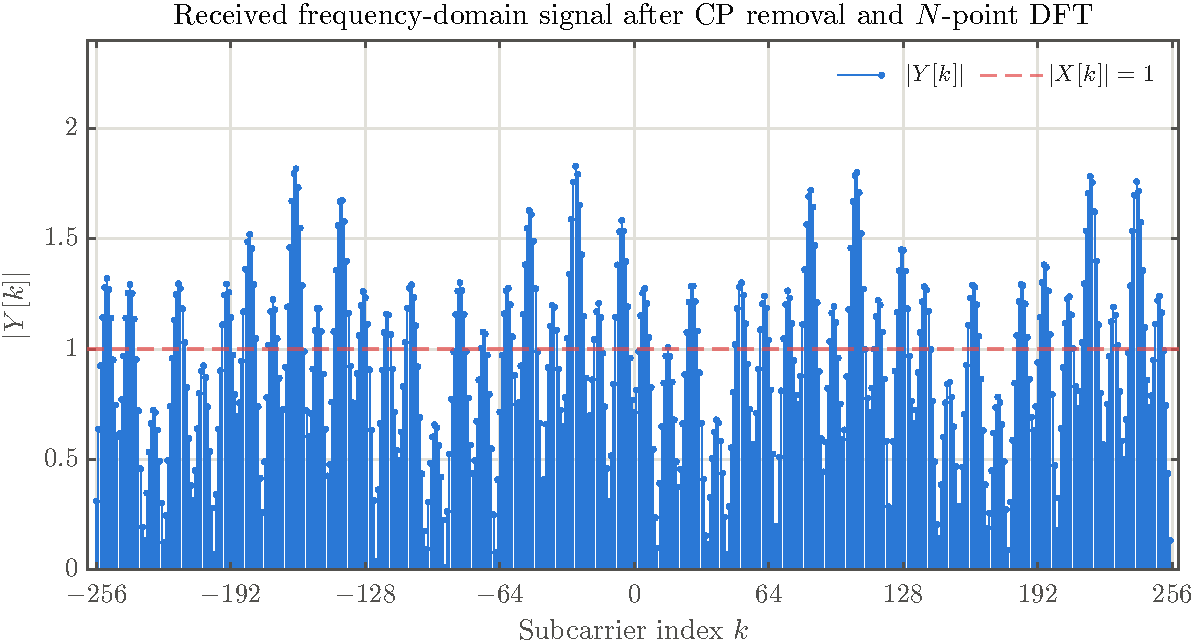
\includegraphics[width=0.92\linewidth]{q4b2.pdf}
    \caption{Magnitude of the Received Frequency-Domain Signal $Y[k]$}
\end{figure}

$|Y[k]|$ has exactly the shape of $|H[k]|$ in Q3(c). Part (c) shows that $Y[k] = H[k]X[k]$, and QPSK has
$|X[k]| = 1$ (red dashed line), so $|Y[k]| = |H[k]|$; the data only rotates each subcarrier. Subcarriers in a deep
fade, such as $k = -90$ with $|Y| = 0.009$, arrive almost erased. With noise they would fail first, which is why real
OFDM systems spread channel coding across subcarriers. The mean of $|Y[k]|^2$ over the symbol is 1.000, which again
matches $\sum_i |h_i|^2 = 1$.

\newpage

\section{(c) Channel Estimate $H[k] = Y[k]/X[k]$}

\question{Please calculate
\[ H[k] = \frac{Y[k]}{X[k]} \]
Draw the magnitude of the frequency domain response $H[k]$ (10\%). Observe this figure and the figure in Q3(c). Are
they the same or not the same? Please explain the reason. (5\%)}

Dividing by the known data removes the QPSK phases. The top panel shows $|Y[k]/X[k]|$ as stems together with the
Q3(c) values $|H(f_k)|$ as black circles (every 4th subcarrier, to keep the plot readable); the phase is shown below it.

\textbf{They are the same.} Over all 512 subcarriers the largest difference between $Y[k]/X[k]$ and $H(f_k)$ from
Q3(c) is $7.9 \times 10^{-15}$, which is only rounding error. Two facts are needed for this.

\textbf{1) The CP turns linear convolution into circular convolution.} The kept samples are
\begin{equation}
    y[N_g + n] = \sum_{l=0}^{L-1} h[l]\,x_{\mathrm{cp}}[N_g + n - l], \qquad n = 0, \ldots, N-1 .
\end{equation}
Because $l \le L - 1 = 50 \le N_g = 64$, the index $N_g + n - l$ never drops below 0. When it falls inside the CP, the
CP supplies $x[(n - l) \bmod N]$, which is the value a circular convolution would use. Hence
\begin{equation}
    y[N_g + n] = \sum_{l} h[l]\,x[(n - l) \bmod N] = (h \circledast x)[n],
\end{equation}
and the script confirms it (difference $1.4 \times 10^{-15}$). By the DFT convolution theorem,
$Y[k] = H_N[k]\,X[k]$ with $H_N[k] = \sum_n h[n] e^{-j2\pi kn/N}$, the $N$-point DFT of $h[n]$. Each subcarrier is
multiplied by one complex number and nothing leaks in from the other subcarriers.

\textbf{2) The DFT of $h[n]$ equals $H(f)$ at the subcarriers.} The delays lie exactly on the sample grid
($\tau_i = n_i/F_s$ with integer $n_i$), so
\begin{equation}
    H_N[k] = \sum_{i} h_i\,e^{-j2\pi k n_i/N} = \sum_i h_i\,e^{-j2\pi (k F_s/N)\tau_i} = H(f_k).
\end{equation}
Together, $Y[k]/X[k] = H(f_k)$ exactly. Nothing else in this setup could make them differ: there is no noise, the
channel is constant over the symbol, and transmitter and receiver use the same DFT size and sample timing.

\textbf{When they would differ.} The bottom panel reruns the whole chain with other CP lengths. With $N_g = 50$ and
$64$ the error stays at the rounding level. With $N_g = 49$ the 200\,ns path reaches one sample beyond the CP and the
error jumps to $5.85 \times 10^{-3}$ on every subcarrier; only one received sample is wrong, so the error is an impulse
in time and flat across $k$. With $N_g = 32$, 18 samples of the last path fall outside the CP and the error grows to
0.15. The circular-convolution property is gone, energy leaks between subcarriers (ICI), and $Y[k]/X[k]$ no longer
equals the channel response. This confirms the bound $N_g \ge L - 1 = 50$ from Q1(d) and Q3(a). The two figures would
also differ if the path delays were not multiples of $T_s$, because then the sampled channel spreads over many taps and
$H_N[k]$ only approximates $H(f_k)$. With receiver noise, $Y/X$ would become a noisy estimate, worst at faded
subcarriers such as $k = -90$.

\begin{figure}[H]
    \centering
    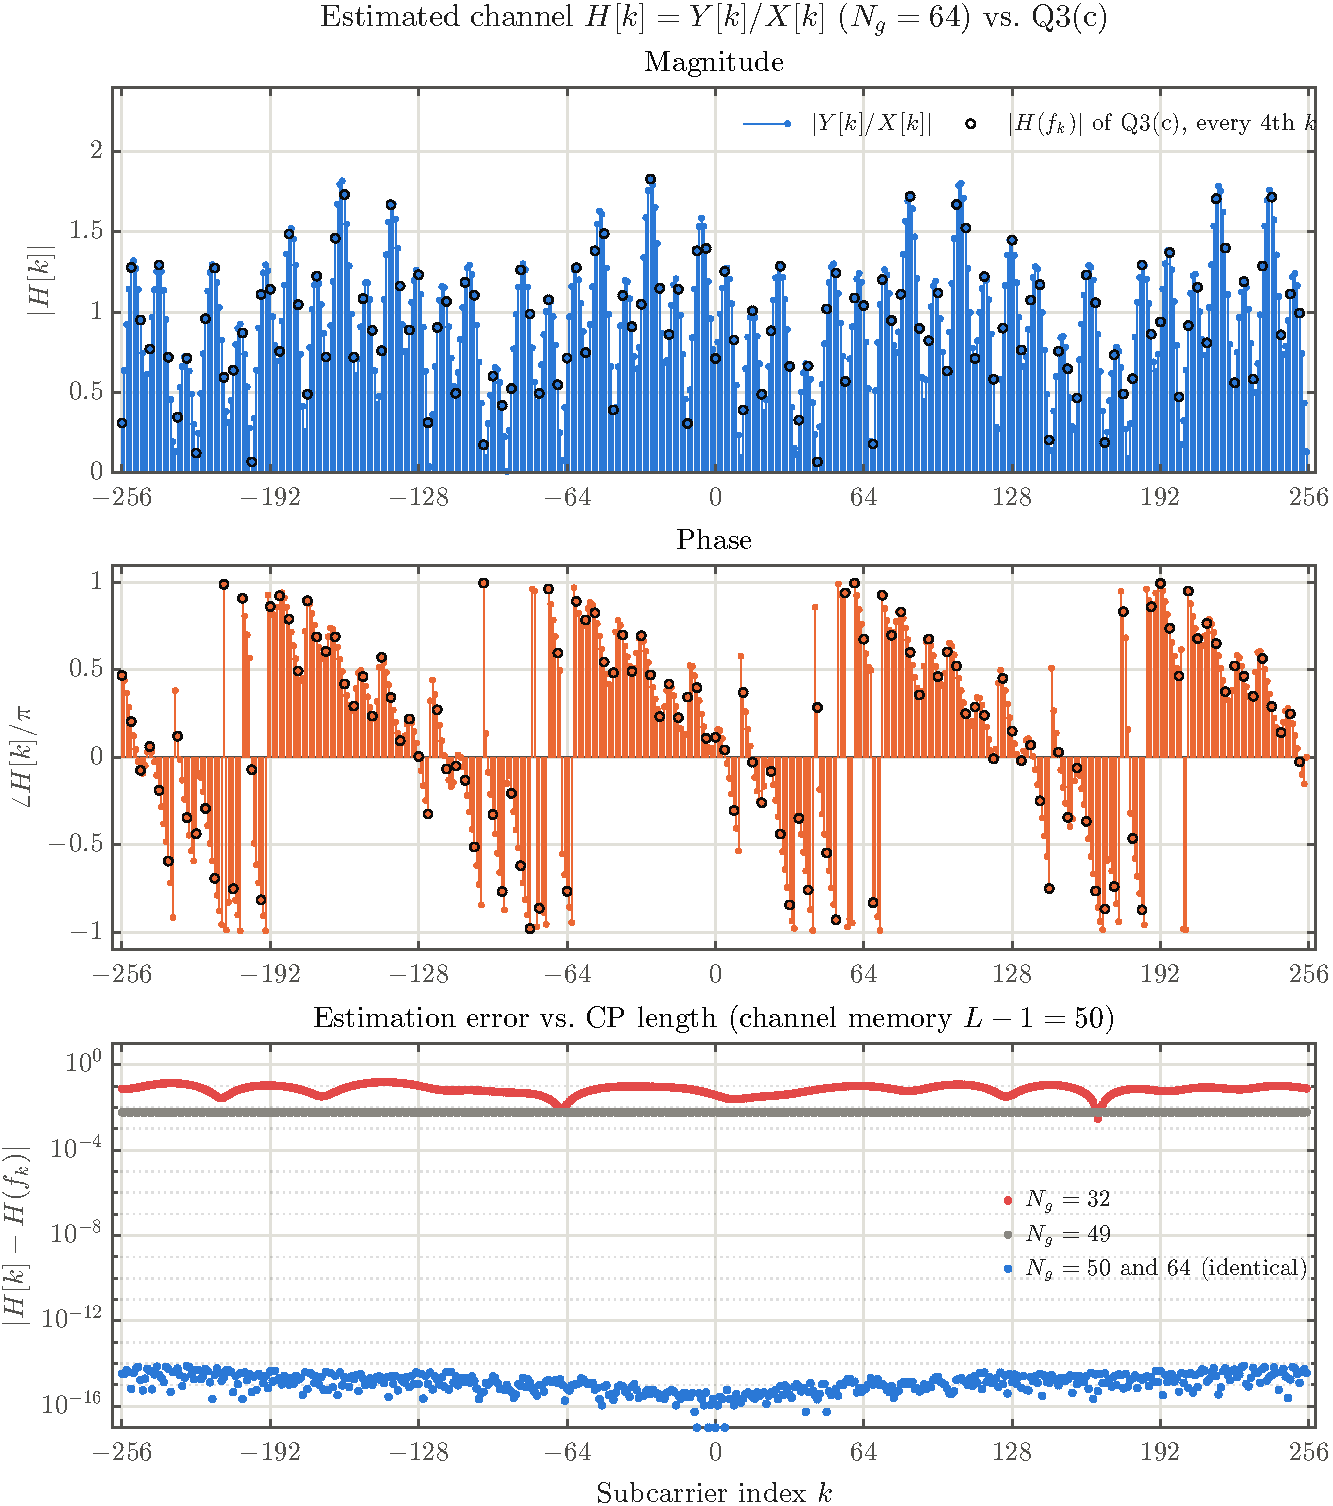
\includegraphics[width=0.88\linewidth]{q4c.pdf}
    \caption{Estimated $H[k] = Y[k]/X[k]$ (stems) vs.\ $H(f_k)$ from Q3(c) (circles), and the Estimation Error for Different CP Lengths}
\end{figure}

\newpage

% ─────────────────────────────────────────────
\chapter{AI Tool Disclosure}
\label{ch:ai}
% ─────────────────────────────────────────────
\question{Please disclose how you use AI tools and its version.}

I used \textbf{Claude Opus 5.5} to help with this homework in the following four parts:
\begin{enumerate}[label=(\arabic*)]
    \item Understanding the homework specification.
    \item Assisting with the MATLAB code.
    \item Plotting the figures.
    \item Writing this \LaTeX{} report.
\end{enumerate}

\end{document}
